The population synthesis for the detections of the double compact objects (DCOs) was performed using the Compact
Object Mergers: Population Astrophysics and Statistics (COMPAS; ~\cite{stevenson2017formation, Riley2022,
    Vigna2018}) suite.
COMPAS is a rapid stellar evolution suite and can evolve both single and binary stars following the details outlined
by~\cite{Hurley2000, Hurley2002}.
A list of selected papers that make use of the COMPAS suite is also available on the COMPAS website.\footnote{\url{https://compas.science/science.html}}

This study makes use exclusively of the binary star evolution (BSE) synthesis method.
The default parameters used by the COMPAS software are listed in table 1 in the COMPAS paper~\cite{Riley2022}.

Except for supernova mass remnant prescription, initial eccentricity ($e_i$), metallicity ($z$), and pulsar evolution, all other parameters were taken at the default value.
For a one-to-one correspondence between the two generated data sets, the seed numbers were kept constant.

For the mass of primary star, we draw the values from Kroupa initial mass function (IMF) with $m_1 \in [5, 150]\,\text{M}_\sun$~\cite{kroupa2001variation}.

For the secondary star, we randomly draw from uniform distribution to satisfy $q\equiv m_2/m_1$, where $q\,\in\,[0, 1]$~\cite{sana2012binary}.
An additional constraint of $m_2 \geq 0.1\,m_1$ was placed on $m_2$ as this is the minimum mass necessary for a star to be considered as a main sequence star.

For the semi-major axis of the binary, we drew the parameter values from a flat-in-the-log distribution with $a_i \in [0.1, 1000]\,$AU, such that
$p(a_i) \propto 1/a_i$~\cite{opik1924photographic}.

For the remnant mass prescription, we first considered the Fryer delayed model~\cite{Fryer2012}.
However, this resulted in a concentration of NS mass around $\sim1.28\,\text{M}_\sun$.
To avoid this concentration of NS final mass, we used Müller \& Mandel prescription (M\&M)~\cite{Mandel2020}.
M\&M is a stochastic remnant mass model that offers a smoother mass distribution for NS\@.
We also switched the \textbf{evolve\_pulsar} flag to \textbf{True} during population synthesis.

For metallicity, we drew the values from a $\text{Beta}(5, 80)$ distribution.
The main motivation behind the selection of such biased distribution is the higher metallic content of present-day stars.
The population III stars were primarily composed of pure hydrogen and their deaths produced heavier metals in the Universe.
By this extension, the stars that are present now or those that will merge now must have higher metallic content.
As such, we also note that having stars with higher metallic content might produce more NSNS or NS-BH pairs for detection.

For eccentricity, we make use of two cases,
\begin{itemize}
    \item Case I: All the binary systems are generated using a flat distribution, $e \in [0, 1]$.
    \item Case II: All the binary systems are generated with circular orbits, i.e., $e = 0$.
\end{itemize}

Details about the selection of metallicity and eccentricity values in COMPAS are provided in appendix~\ref{sec:appA}.

\subsection{Milky way Model}
\label{subsec:mw}
In this section, we will briefly outline the milky way galaxy model used in this study.
The model is developed by~\cite{wagg2021gravitational} and makes use of the galaxy's enrichment history by taking
into account the metallicity-radius-time relationship~\cite{Frankel2018}.
It uses a separate star formation history and spatial distribution for the \lowalpha, \highalpha\ discs, and bulge in the galaxy.

\paragraph*{\textbf{Star formation rate}}
The star formation rate for both the \lowalpha\ and \highalpha\ disks is expressed as,
\begin{equation}
    p(\tau) \propto \exp\left(-\frac{\tau_m - \tau}{\tau_\text{SFR}}\right),
    \label{eq:star_formation_rate_equation}
\end{equation}
where $\tau$ is the time difference between the star's ZAMS stage and today.
The age of milky way galaxy, $\tau_m$, is taken as \SI{12}{\giga\yr}, and the star formation rate as, $\tau_\text{
    SFR}\ $= \SI{6.8}{\giga\yr}.
The star-forming period of \lowalpha\ and \highalpha\ discs were taken as \SIrange{0}{8}{\giga\yr} and \SIrange{8}{12}{\giga\yr} respectively.
The model adopts \SIrange{6}{12}{\giga\yr} as the star-forming period of the bulge~\cite{Bovy2019}.

\paragraph*{\textbf{Radial distribution}}
The radial distribution of stars within the milky way galaxy was performed using the following expression,
\begin{equation}%
    p(R) = \exp\left(-\frac{R}{R_d}\right)\frac{R}{R_d^2}
    \label{eq:radial_distribution_of_stars}
\end{equation}%

However, a different scale length, $R_d$, was chosen for each component of the galaxy.
For \lowalpha, the model uses $R_\text{exp}(\tau)$ as the scale length~\cite[Eq 6]{Frankel2018}, where

\begin{equation}%
    R_\text{exp}(\tau) = 4\,\text{kpc}\left[1 - \alpha_{R_\text{exp}}\left(\frac{\tau}{8\,\text{Gyr}}\right)\right],
    \label{eq:exponential_radius_equation}
\end{equation}%
with the value of inside-out growth parameter, $\alpha_{R_\text{exp}}$, as 0.3. For \highalpha\ disc and bulge, the value of scale length was chosen as $(1/0.43)\,$\si{\kpc} and \SI{1.5}{\kpc} respectively.

\paragraph*{\textbf{Vertical distribution}}
The model employs a similar method of single exponent expression with varying scale height parameters for the vertical distribution as well.
The exponential expression used is,
\begin{equation}
    p(|z|) = \frac{1}{z_d}\exp\left(-\frac{z}{z_d}\right),
    \label{eq:vertical_distribution_of_stars}
\end{equation}
where $z$ here is the vertical displacement from the galactic plane.
The scale height parameter, $z_d$, for \lowalpha, \highalpha\ and bulge was taken as \SI{0.3}{\kpc}~\cite{McMillan2011}, \SI{0.95}{\kpc}~\cite{Bovy2016}, and \SI{0.2}{\kpc}~\cite{Wegg2015} respectively.

\subsubsection*{\textbf{Metallicity-radius-time relationship}} The MRT relationship plays an important part, both in the galaxy model and later on in the placement of DCOs within the galaxy as well.
The model makes use of~\cite[Eq. 7]{Frankel2018},
\begin{equation}
    \begin{aligned}
        \feh(R,\tau) = {} & F_m + \nabla\feh R \\
        & - \left(F_m + \nabla\feh R_{\feh=0}^{\text{now}}\right) f(\tau)
    \end{aligned}
\end{equation}

\subsection*{\textbf{Galaxy synthesis:}}
For the synthesis of an instance of the Milky Way galaxy, the model described previously samples the following parameters,
\begin{equation*}
    \theta_i = \{\tau, D, z, \text{component}\},
\end{equation*}
where $\tau$ is the look-back time for the binary, $D$ is the distance from Earth, $z$ is the metallicity, and `component` is the component of the galaxy in which the binary resides.\footnote{One of the three, \lowalpha\ disc, \highalpha\ disc, or bulge.} The parameters are generated for $i = 1, 2, 3, \ldots$, $N_\text{GAL}$, where $N_\text{GAL} = 100$.

\noindent [\textbf{need the codes from Nazeela to further write this section}]

\subsection{Parameters of interest}
We first generated \num{1e7} values for metallicity using the beta distribution within the COMPAS limits (see, appendix~\ref{sec:appA} for details).
The values were stored in ten separate grid files and used with COMPAS to simulate the binaries.
We denote the zero-age main sequence (ZAMS) parameters of the binaries as,
\begin{equation}%
    \mone{ZAMS}, \mtwo{ZAMS}, \semaxis{ZAMS}, \ecc{ZAMS}, z, \o
\end{equation}%

COMPAS evolves the binaries up to \SI{13.7}{\giga\yr}.
We represent the resulting double compact object (DCO) parameters as,
\begin{equation}%
    \mone{DCO}, \mtwo{DCO}, \semaxis{DCO}, \ecc{DCO}, \interval{evolve}, \interval{inspiral}, \interval{light}, z, \o,
\end{equation}%
where $z$ is the metallicity of the binary system, $\o$ is the seed number, $\interval{evolve}$ is the time required to form DCO from ZAMS, and $\interval{inspiral}$ is the DCO in-spiral time. $\semaxis{ZAMS}$, $\semaxis{DCO}$, $\ecc{ZAMS}$, and $\ecc{DCO}$ are the semi-major axis and eccentricity of the binary orbit at ZAMS and DCO formation respectively.
We also consider a third time interval, $\interval{light}$ as the time required for gravitational waves (GWs) from
the merged binary to reach the detector (see, figure~\ref{fig:binaryevolution}). To calculate $\interval{light}$ we
need to know the distance to that particular binary, this was done using the galaxy model provided by~\cite{
    wagg2021gravitational}, see section~\ref{subsec:mw}.
\begin{figure}[!ht]%
    \centering
    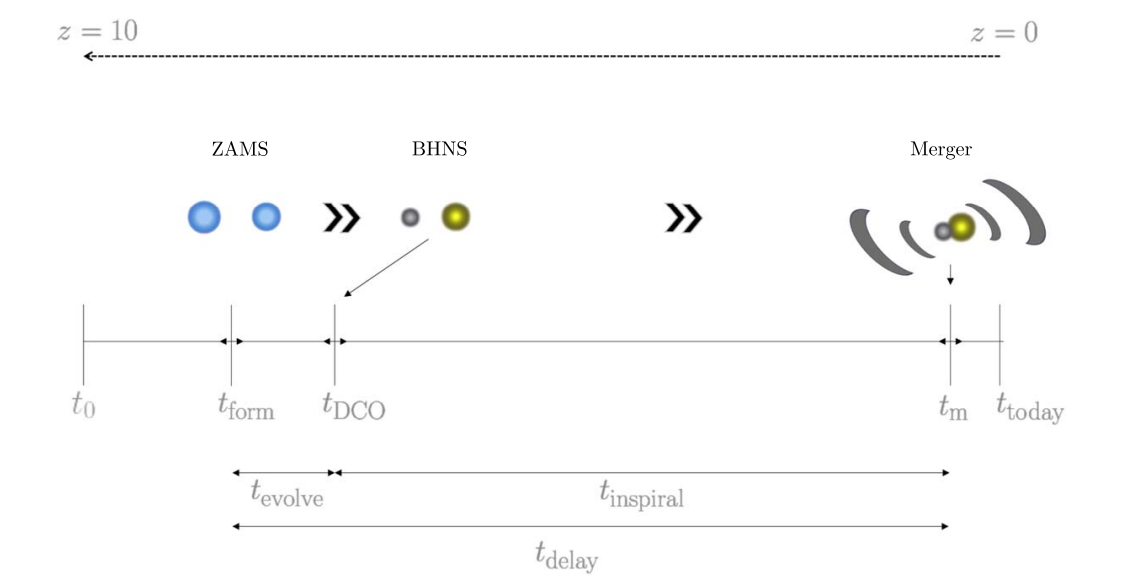
\includegraphics[width=\linewidth]{images/binary_evolution}
    \caption{Schematic diagram showing various time intervals for a binary system from ZAMS formation, to DCO, and merger. The interval between merger and present is taken as $t_\text{light}$. The figure is taken from~\cite{Riley2022}.}
    \label{fig:binaryevolution}
\end{figure}%

These parameters were then provided to the python framework LEGWORK~\cite{wagg2021legwork} that evolved these binaries from the DCO stage to the merger state.
This package evolves the binaries using equation from~\cite{Peters1963, Peters1964}.
The detection is made based on the signal-to-noise ratio (SNR) of the binary averaged over sky position, polarization, and orientation using the following expression from~\cite{Finn2000},
\begin{equation}
    \rho^2 = \sum_{n=1}^{\infty}\int_{f_{n, i}}^{f_{n, f}}\frac{h_{c, n}^2}{f_n^2 S_n(f_n)}\,\text{d}f_n,
\end{equation}
where $n$ is the GW harmonic, $f_n$ represents the orbital frequency of $n^\text{th}$ harmonic.
The parameter $S_n(f_n)$ is the LISA sensitivity curve function~\cite{Robson2019}, and $h_{c, n}$ is the characteristic strain of the $n^\text{th}$ GW harmonic~\cite{Barack2004}.
\begin{equation}
    h_{c,n}^2 = \frac{2^{5/3}}{3\pi^{4/3}}\frac{(G\mathcal{M}_c)^{5/3}}{c^3 D_L^2}\frac{1}{f_\text{orb}^{1/3}}\frac{g
        (n, e)}{nF(e)}
\end{equation}

We use a modified version of the script originally provided by~\cite{wagg2021gravitational} for DCO detections.
The modified script

\subsection{Detection}\label{subsec:d}

\subsection{Model variation} \label{subsec:mv}
In all the previous research, $e_\text{ZAMS}$ was taken as $0$~\cite{Vigna2018, Barrett2018, Lau2020, Broekgaarden2021, wagg2021gravitational}.
The main reason for this assumption is that they argue that eccentricity at ZAMS is not likely critical for predicting detection rates as they deal with post-interaction binaries and their orbital eccentricities become zero after mass transfer~\cite{Hurley2002}. %, de2015merger}).
To test the accuracy of this assumption, we simulate another population with the same parameters.
The only change is that $e_\text{ZAMS}$ of the binaries is left to be varied by the COMPAS suite.
We compare the difference in detection rates and properties of the two models and give our conclusion.

\subsection{Binary Evolution}\label{subsec:be}
One of the most important factors in the observation of any source is their distance from the observational instrument.
As it is a known fact that for all the sources, we can observe their past depending upon how far are we from it.
This surely complicates the evolution of our DCO as at the time of observation, LISA will also be observing the past of the sources.
To handle such a situation, we first calculate the time the GW will take from the source to LISA using the given distances within the milky way.
This logic is implemented within Legwork~\cite{wagg2021legwork} which gives strong tools for evolving the sources to the desired point.